\documentclass[a4paper]{article}
\usepackage[T1]{fontenc}
%\usepackage{times, mathptm}
\usepackage[scaled]{luximono}
\usepackage{utopia}
\usepackage[adobe-utopia]{mathdesign}
\usepackage{a4wide}
\usepackage{comment}
\usepackage{bcprules}
\usepackage{waebric}
\usepackage{sdf}
\usepackage{xspace}
\usepackage{url}
\usepackage{float}
\usepackage{epsfig}
\usepackage{listings}
\usepackage{amsmath}
\usepackage{mathpartir}
\usepackage{wasysym}
\usepackage{stmaryrd}




\def\waebric{\textsc{Waebric}\xspace}
\def\Waebric{\textsc{Waebric}\xspace}
\def\V#1{\ensuremath{\mbox{\textit{#1}}}}
\def\concat{+}
%\def\concat{\ensuremath{\;\text{+\hspace{-0.6ex}+}\;}}
\def\tostring#1{\ensuremath{\lfloor #1\rfloor}}
%\def\tostring#1{\ensuremath{\llbracket #1 \rrbracket}}

\def\asfsdf{\asf+\-\sdf}
\def\asf{\textsc{Asf}}
\def\sdf{\textsc{Sdf}}

% TODO: use listings
\def\Def{\textbf{def}}
\def\End{\textbf{end}}
\def\If{\textbf{if}}
\def\Each{\textbf{each}}
\def\Else{\textbf{else}}
\def\Yield{\textbf{yield}}
\def\Echo{\textbf{echo}}
\def\Module{\textbf{module}}
\def\Var#1{\textit{#1}}
\def\Site{\textbf{site}}


\floatstyle{boxed}
\newfloat{semantics}{thp}{lop}
\floatname{semantics}{Figure}


\begin{document}
\title{\waebric: a Little Language for Markup Generation}
\author{Tijs van der Storm}
\date{\today}
\maketitle

\begin{abstract}
  \noindent \waebric\ is a small language for generating XHTML
  markup. Its design is motivated by the lack of programmer friendly
  abstraction facilities in existing markup languages.  \waebric\
  provides a user-friendly syntax to factor Web pages in
  self-contained functional building-blocks. This report introduces
  and motivates \waebric, and presents its syntax and semantics.
\end{abstract}

\section{Introduction}

\subsection{Motivation}

\begin{itemize}
\item (X)HTML is too verbose to be typed (or read) by humans.
\item Template languages feature elaborate quoting schemes that make
  designing templates form (X)HTML even more cumbersome.
\item Template languages often do not allow functional abstraction
  and/or recursion.
\item Template languages do not support ``around'' parameterization
  where one can reuse a piece of markup with one or more holes in it.
\item Template languages often allow arbitrary computation thus
  violating separation of concerns guidelines.
\item WYSIWYG editors have their own issues like generating
  inaccessible and unmaintainable XHTML code.
\end{itemize}



\subsection{What \waebric offers}

\waebric is a small programming language to factor web pages in
reusable, function building blocks. Concretely, this amounts to the
following:
\begin{itemize}
\item A \waebric program consists of a number of function
  declarations. A function may accept a number of parameters and
  produces a piece of markup. Functions can be recursive.
\item Markup is produced using (pre-defined) ``function calls''
  corresponding to the tags that are part of XHTML 1.1. Keyword
  parameters to these functions correspond to XML attributes of the
  tag in question.
\item The builtin operators \textbf{echo}, \textbf{comment},
  \textbf{cdata} are used to produces text content, XML comments, and
  CDATA sections respectively.
\item Limited control flow is provided through the
  \textbf{if}/\textbf{else} and the \textbf{each} iteration
  construct. Both these constructs operate on expressions (i.e. data,
  \textit{not} markup).
\item The special statement \textbf{yield} is provided to parameterize
  functions with additional markup. Markup arguments to a function
  invokation will be output where (one or more) \textbf{yield} is
  encountered. This mechanism is similar to (but weaker than) how Ruby
  block arguments are used in Markaby\footnote{\url{http://markaby.rubyforge.org/}}.
\item \waebric provides special syntax for common attributes in XHTML,
  such as ``class'' and ``id''. This is inspired by
  \textsc{Haml}\footnote{\url{http://haml.hamptoncatlin.com/}}.
\end{itemize}

In the design of \waebric, explicit care is taken that \textit{data}
can be output as markup, but markup can \textit{never} act as
data. Thus it is not possible to ``compute'' with generated
markup. Furthermore, to enforce strict model-view separation,
computation with data is limited to testing the type or presence of
data and looping through data using \textit{each}.


\section{Syntax}

\subsection{A Simple Example}

A \waebric file always starts with the keyword \textbf{module}
followed by an identifier that should correspond to the basename of
the file. A typical  \waebric program looks as follows:
\begin{quote}
\begin{lstlisting}[language=waebric]
module homepage

site 
  index.html: home("Hello World!")
end

def home(msg)
  html {
    head title msg;
    body echo msg;
  }
end
\end{lstlisting}
\end{quote}
This program should be in a file called \texttt{homepage.wae}. This
module contains one site definition that states that
\texttt{index.html} should contain the output of evaluating the
function \texttt{home} with a single, string-valued argument.

If we look at the \texttt{home} function, we see that it constructs a
standard HTML document containing a header with a title element and a
body. Both the contents of the title element and the body will be the
value passed in as \texttt{msg}. Since \texttt{html} is not defined in
this module and since it is not imported either, \waebric assumes it
is part of XHTML 1.1 and will output the corresponding tags. Within
those tags, it will generate the output of the statements enclosed in
curly braces. 

The \texttt{html, head, title, body} elements in the example are
called \textit{markup} statements (or just \textit{markup}). Markup
can be nested by juxtaposing function calls and/or standard element
names. For instance, the title element (containing msg) will be
contained in the head element. The last item in a sequence of markups
can be a statement or an expression. An example of the former is the
block enclosed in curly braces which is passed into the html
element. The nesting of msg in the title element is an example of the
latter.

\subsection{Embedding}


\subsection{Caveat}

Some notes are in order with respect to how markup juxtaposition is
parsed in \waebric. Basically, it boils down to the following two
observations. First, an single identifier interpolated in a string is
parsed as an expression whereas a single identifier in a statement
context is parsed as markup (e.g. a function call or an XHTML element
construction). Secondly, an identifier in the last position of a
markup chain/spine is parsed as a variable (not as markup). The
following examples illustrate these rules:
\begin{quote}
\begin{lstlisting}[language=waebric]
p;              // markup
p p;            // markup, variable
p p();          // markup, markup
echo "<p>";     // variable
echo "<p()>";   // markup
echo "<p p>";   // markup, variable
echo "<p p()>"; // markup, markup
\end{lstlisting}
\end{quote}
As the example shows, parentheses can be used to force the parser to
see an identifier as markup.


\subsection{Data}

It is not possible to compute with data in \waebric, however, you can
create and inspect data to a certain extent. \waebric contains literal
syntax for numbers, strings, symbols, lists and records (inspired by
JSON\footnote{\url{http://www.json.org/}}). Some examples are listed below:
\begin{quote}
\begin{lstlisting}[language=waebric]
123 // a number
"abc" // a string
'sym // a symbol
[123, "abc", 'sym] // a list
{ name : "John Smith", age: 30 }  // a record
\end{lstlisting}
\end{quote}

The inspection of data is limited to testing whether an expression is
of list or record type using $x$.list? and $x$.record? respectively,
and obtaining a field of a record the using the dot-notation
$x.y$. Testing the type of an expression can only occur in the
condition of an if-statement. Finally,  lists can be iterated through
using the \textbf{each} statement.

\subsection{Yield}

In the example above, the html markup-invocation receives a block
enclosed in curly braces that will be the content of the
\verb!<html></html>! element. Users can define functions that exhibit
the same behaviour using yield. Consider the following refactoring of
the example above:
\begin{quote}
\begin{lstlisting}[language=waebric]
def home(msg)
  layout(msg) echo msg;
end

def layout(title)
  html {
    head title title;
    body yield;
  }
end
\end{lstlisting}
\end{quote}
The home function now calls an auxiliar function (layout) which
receives the statement \texttt{\textbf{echo} msg} as
block-argument. The layout function inturn sets up a basic HTML
skeleton (with the title argument as title) passes the
\texttt{\textbf{yield}} statement to the body-tag. This has the effect
that in the invocation of layout above, the output of
\texttt{\textbf{yield}} will be equal to the output of
\texttt{\textbf{echo} msg}.

Although the input-output behaviour of \texttt{home} is exactly the
same as it was before, the page-skeleton as embodied in the layout
function can now be reused in the generation other pages.


\subsection{Attributes}

\subsubsection{Introduction}

Both function calls and markup elements can receive parameters. They
come in two forms:
\begin{enumerate}
\item $f(x_1 = a_1,..., x_n = a_n)$: if $f$ is a tagname (for instance
  ``div''), $x_1,...,x_n$ are interpreted as XML attributes. The
  values are obtained from the values of the $a_1,...,a_n$
  respectively. In the case of a function calls, the keywords are
  ignored, and $a_1,...,a_n$ is passed as an ordinary list of
  arguments (see 2 below).
\item $f(a_1,..., a_n)$: if $f$ is a defined function, $a_1,...,a_n$ are its
  arguments. In the case of markup (for instance if $f$ is actually
  the tagname ``input''), the list $a_1,...,a_n$ is translated to the
  the keyword parameter list $\text{value} = a_1, ..., \text{value} =
  a_n$. In the case that $n > 1$ the value of ``value'' attribute is
  taken to be the value of the last keyword argument.
\end{enumerate}

\subsubsection{Shorthands}

\waebric provides shorthand notation for common XHTML attributes
(inspired by Haml). See Table~\ref{TBL:shorthand} for an overview of
how this shorthand notation corresponds to regular attribute
specification.

\begin{table}
\begin{center}
\begin{tabular}{|l|l|}\hline
\textbf{Shorthand} & \textbf{Equivalent longhand} \\\hline\hline
div.$x$ & div(class=$x$)\\\hline
div\#$x$ & div(id=$x$)\\\hline
input\$$x$ & input(name=$x$)\\\hline
input:$x$ & input(type=$x$)\\\hline
img@$w$\%$h$ & img(width=$w$, height=$h$)\\\hline
\end{tabular}
\end{center}
\caption{Meaning of attribute shorthands\label{TBL:shorthand}}
\end{table}

The syntax of shorthands accepts identifiers as variable part (except
for the @-attribute which accepts natural numbers). The height part of
the @-attribute is optional. Shorthands can be combined. For instance:
p\#intro.dropcaps combines the shorthands for the id and class
attributes.


\subsection{Recursive Menus}

\begin{figure}
\begin{quote}
\begin{minipage}{0.6\linewidth}
\begin{lstlisting}[language=waebric]
def menu(menu)
  echo menu.title;
  ul each (kid: menu.kids) 
       menu-item(kid);
end

def menu-item(item)
  if (item.kids)
    li menu(item);
  else
    li a(href=item.link) item.title;
end
\end{lstlisting}
\end{minipage}
\begin{minipage}[b]{0.4\linewidth}
\begin{center}
\fbox{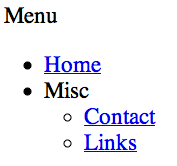
\epsfig{file=Generated-Menu,width=0.5\linewidth}}
\end{center}
\end{minipage}
\end{quote}
\caption{Recursive menus in \Waebric\ and the possible
  output\label{FIG:menus}}
\end{figure}

The example in Figure~\ref{FIG:menus} shows how recursive menus could
be defined in \Waebric. The first function, menu, receives a data
object (\Var{menu}) containing the labels, URLs and sub-menus that
should be rendered in XHTML. The next statement just renders the title
of the (current) menu using the built in statement echo. After
the title follows an unordered list containing the items of this
menu. For each element in the ``kids'' property of \Var{menu} the
menu-item function is called.

The menu-item function first checks whether this \Var{item} has any
children (sub-menus). If so, it produces a li(st) element containing
the output of a recursive call to menu. If there are no sub-menus,
the result is a list element with an anchor tag which links the title
of item to its URL. The result of an invocation (with the appropriate
data for the \textit{menu} parameter) of menu could look like the
screen shot next to the source code.


\begin{comment}

\section{Semantics}


\subsection{Abstract Syntax}

See Figure~\ref{FIG:abstract-syntax}.

\def\NT#1{\ensuremath{\mathsf{#1}}}
\begin{figure}
\begin{minipage}[t]{0.33\linewidth}\small
\[
\begin{array}{rcl}
S_i \in \NT{S} & ::= & \text{\textbf{echo} }\NT{E} \\
& | & \text{\textbf{comment} }\V{String} \\
& | & \text{\textbf{cdata} }\NT{E}\\
& | & \text{\textbf{yield}}\\
& | & \text{\textbf{if} }(\NT{P})\;\NT{S} \text{ \textbf{else} }\NT{S}\\
& | & \text{\textbf{each} }(x: \NT{E})\;\NT{S}\\
& | & \text{\textbf{let} }\NT{B}\text{ \textbf{in} }\NT{S}\text{ \textbf{end}}\\
& | & \NT{S}; \NT{S}\\
& | & \NT{M}\; \NT{S}\\
& | & \NT{M}\; \NT{E}\\
& | & \NT{M}
\end{array}
\]
\end{minipage}
\begin{minipage}[t]{0.33\linewidth}\small
\[
\begin{array}{rcl}
M_i \in\NT{M} & ::= & \NT{M}\;\NT{M}\\
& | & f_n(\NT{E}_1,...,\NT{E}_n)\\
& | & t_n(x_1 = \NT{E}_1,...,x_n =\NT{E}_n)\\
e_i \in \NT{E} & ::= & x \\
& | & \V{Text} \\
& | & [\NT{E}_1,...,\NT{E}_n]\\
& | & \{x_1: \NT{E}_1, ..., x_n: \NT{E}_n\}\\
I_i\in \NT{I} & ::= & \V{Text} \langle \NT{M}\; \NT{E} \rangle \NT{I}\\
  & | & \V{Text} \langle \NT{E} \rangle \NT{I}\\
  & | & \V{Text}
\end{array}
\]
\end{minipage}
\begin{minipage}[t]{0.33\linewidth}\small
\[
\begin{array}{rcl}
B_i\in \NT{B} & ::= & x = \NT{E} \\
& | & f_n(x_1, ..., x_n) = \NT{S}\\
& | & \NT{B} ; \NT{B}\\
p_i \in \NT{P} & ::= & \NT{E}\\
& | & \NT{E}.\text{\textbf{record?}}\\
& | & \NT{E}.\text{\textbf{list?}}\\
& | & !\NT{P} \\
& | & \NT{P}\; \&\&\; \NT{P}\\
& | & \NT{P}\; ||\; \NT{P}\\
\end{array}
\]
\end{minipage}
\caption{Abstract syntax of \waebric\label{FIG:abstract-syntax}}
\end{figure}

\subsection{Semantics}


Semantic domains

Values:
\[
\begin{array}{rcl}
v_i \in \NT{V} &::=& \mathbb{N} \;|\; \V{String} 
\;|\; [\NT{V}_1, ..., \NT{V}_n] \;|\; \{x_1: \NT{V}_1, ..., x_n: \NT{V}_n\}\\
c_n \in \NT{F} &::=& \lambda x_1,...,x_n\; \NT{S}\\
C_i \in \NT{C} &:& \NT{VE} \times\NT{FE} \times\NT{F}\\
\Gamma \in \NT{VE} &:& \NT{X}\rightarrow\NT{V}\\
\Lambda \in \NT{FE} &:& \NT{X}\rightarrow\NT{C}\\
\end{array}
\]


\[
\tostring{\_}: \NT{V} \rightarrow \V{String}
\]


Figure~\ref{FIG:semantics} shows a natural semantics of \waebric.

\begin{semantics}\small
\begin{mathpar}
\inferrule*[right=Var]{
\Gamma(x) = v
}{
\Gamma, \Lambda \vdash_E x \rightarrow v
}

\inferrule*[right=Atom]{ 
}{
\Gamma, \Lambda \vdash_E a \rightarrow \llbracket a\rrbracket
}

\inferrule*[right=List]{ 
1 \leq i \leq n\\
\Gamma, \Lambda \vdash_E e_i \rightarrow v_i
}{
\Gamma, \Lambda \vdash_E [e_1,...,e_n] \rightarrow 
[v_1, ..., v_n]
}

\inferrule*[right=Record]{ 
1 \leq i \leq n\\
\Gamma, \Lambda \vdash_E e_i \rightarrow v_i
}{
\Gamma, \Lambda \vdash_E \{x_1: e_1,...,x_n: e_n\} \rightarrow 
\{x_1: v_1, ..., x_n: v_n\}
}

\inferrule*[right=Lookup]{ 
1 \leq i \leq n\\
\Gamma, \Lambda \vdash_E e \rightarrow \{x_1: v_1, ...,x_n: v_n\}
}{
\Gamma, \Lambda \vdash_E e.x_i \rightarrow v_i
}

\end{mathpar}
\caption{Semantics of expressions\label{SEM:expression}}
\end{semantics}

\begin{semantics}\small
\begin{mathpar}
\inferrule*[right=Defined]{
\Gamma, \Lambda \vdash_E e \rightarrow v
}{
\Gamma, \Lambda \vdash_P e
}

\inferrule*[right=IsList]{
\Gamma, \Lambda \vdash_E e \rightarrow [v_1,...,v_n]
}{
\Gamma, \Lambda \vdash_P e.\text{\textbf{list?}}
}

\inferrule*[right=IsRecord]{
\Gamma, \Lambda \vdash_E e \rightarrow \{x_1: v_1,...,x_n: v_n\}
}{
\Gamma, \Lambda \vdash_P e.\text{\textbf{record?}}
}

\inferrule*[right=Or-1]{
\Gamma, \Lambda \vdash_P p_1
}{
\Gamma, \Lambda \vdash_P p_1\;||\;p_2
}

\inferrule*[right=Or-2]{
\Gamma, \Lambda \vdash_P p_2
}{
\Gamma, \Lambda \vdash_P p_1\;||\;p_2
}

\inferrule*[right=And]{
\Gamma, \Lambda \vdash_P p_1\\
\Gamma, \Lambda \vdash_P p_2
}{
\Gamma, \Lambda \vdash_P p_1\;\&\&\;p_2
}

\inferrule*[right=Not]{
\Gamma \not\vdash_P p
}{
\Gamma, \Lambda \vdash_P \;!p
}
\end{mathpar}
\caption{Semantics of predicates\label{SEM:predicates}}
\end{semantics}


\begin{semantics}\small
\begin{mathpar}
\inferrule*[right=echo]{
\Gamma, \Lambda \vdash_E e \rightarrow v
}{
\Gamma, \Lambda, \beta \vdash_S \text{\textbf{echo} }e \rightarrow \tostring{v}
}


\inferrule*[right=Yield]{ 
}{
\Gamma, \Lambda, \beta \vdash_S \text{\textbf{yield}} \rightarrow \beta
}


\inferrule*[right=Comment]{
}{
\Gamma, \Lambda, \beta \vdash_S \text{\textbf{comment} }s \rightarrow
\text{``$<$!$-$$-$''} \concat \tostring{s} \concat \text{``$-$$-$$>$''}
}

\inferrule*[right=CData]{
\Gamma, \Lambda \vdash_E e \rightarrow v
}{
\Gamma, \Lambda, \beta \vdash_S \text{\textbf{cdata} }e \rightarrow
\text{``$<$![CDATA[''} \concat \tostring{v} \concat \text{``]]$>$''}
}

\inferrule*[right=If-1]{
\Gamma, \Lambda \vdash_P p\\
\Gamma, \Lambda, \beta \vdash_S S_1 \rightarrow s_1
}{
\Gamma, \Lambda, \beta \vdash_S \text{\textbf{if} }(p)\; S_1 \text{
  \textbf{else} } S_2 \rightarrow s_1
}

\inferrule*[right=If-2]{
\Gamma, \Lambda \vdash_P\; !p\\
\Gamma, \Lambda, \beta \vdash_S S_2 \rightarrow s_2
}{
\Gamma, \Lambda, \beta \vdash_S \text{\textbf{if} }(p)\; S_1 \text{
  \textbf{else} }S_2 \rightarrow s_2
}

\inferrule*[right=Sequence]{
\Gamma, \Lambda, \beta \vdash_S S_1 \rightarrow s_1\\
\Gamma, \Lambda, \beta \vdash_S S_2 \rightarrow s_2\\
}{
\Gamma, \Lambda, \beta \vdash_S S_1;\; S_2 \rightarrow s_1\concat s_2
}


\inferrule*[right=Each]{
\Gamma, \Lambda \vdash_E e \rightarrow [v_1, ..., v_n]\\
1 \leq i \leq n\\
\Gamma[x/v_i], \Lambda, \beta \vdash_S S \rightarrow s_i\\
}
{
\Gamma, \Lambda, \beta \vdash_S \text{\textbf{each} }(x: e)\; S 
\rightarrow \sum^n_{i = 1} s_i
}

\inferrule*[right=Let]{
\Gamma, \Lambda \vdash_B B \rightarrow \langle\Gamma', \Lambda'\rangle\\
\Gamma', \Lambda', \beta \vdash_S S \rightarrow s
}{
\Gamma, \Lambda, \beta \vdash_S \text{\textbf{let} } B
\text{ \textbf{in} } S \text{ \textbf{end}}\rightarrow s
}

\inferrule*[right=Markup-1]{
\Gamma, \Lambda, \beta \vdash_S S \rightarrow \beta'\\
\Gamma, \Lambda, \beta' \vdash_M M \rightarrow s'
}{
\Gamma, \Lambda, \beta \vdash_S M \; S \rightarrow s'
}


\inferrule*[right=Markup-2]{
\Gamma, \Lambda  \vdash_E e \rightarrow v\\
\Gamma, \Lambda, \tostring{v} \vdash_M M \rightarrow s'
}{
\Gamma, \Lambda, \beta \vdash_S M \; e \rightarrow s'
}

\inferrule*[right=Markup-3]{
\Gamma, \Lambda, \beta \vdash_M M \rightarrow s
}{
\Gamma, \Lambda, \beta \vdash_S M \rightarrow s
}

\end{mathpar}
\caption{Semantics of statements\label{SEM:statements}}
\end{semantics}

\begin{semantics}\small
\begin{mathpar}
\inferrule*[right=Bindings]{
\Gamma, \Lambda \vdash_B B_1 \rightarrow\langle \Gamma_1, \Lambda_1\rangle\\
\Gamma_1, \Lambda_1 \vdash_B B_2 \rightarrow\langle \Gamma_2, \Lambda_2\rangle
}{
\Gamma, \Lambda \vdash_B B_1; B_2 \rightarrow \langle \Gamma_2, \Lambda_2\rangle
}

\inferrule*[right=Bindings-Var]{
\Gamma, \Lambda \vdash_E e \rightarrow v
}{
\Gamma, \Lambda \vdash_B x = e \rightarrow \langle\Gamma[x/v], \Lambda\rangle
}

\inferrule*[right=Bindings-Func]{
C = \langle\Gamma, \Lambda, \lambda x_1, ..., x_n\;S\rangle\\
}{
\Gamma, \Lambda \vdash_B f(x_1, ..., x_n) = S \rightarrow 
\langle\Gamma, \Lambda[f/C]\rangle
}


\end{mathpar}
\caption{Semantics of bindings\label{SEM:bindings}}
\end{semantics}

\begin{semantics}\small
\begin{mathpar}
\inferrule*[right=Nest]{
\Gamma, \Lambda, \beta \vdash_M M_2 \rightarrow \beta'\\
\Gamma, \Lambda, \beta' \vdash_M M_1 \rightarrow s 
}
{\Gamma, \Lambda, \beta \vdash_M M_1\; M_2 \rightarrow s}


\inferrule*[right=Empty]{
f \not\in \text{dom}(\Lambda)\\
}{
\Gamma, \Lambda, \beta \vdash_M f \rightarrow
\text{``$<$''} \concat \tostring{\V{f}}\; \concat \text{``/$>$''}
}


\inferrule*[right=Element]{
t_n \not\in \text{dom}(\Lambda)\\
n > 0\\
1 \leq i \leq n\\
\Gamma, \Lambda \vdash_E e_i\rightarrow v_i\\
s =\sum^{n}_{i = 1} \text{``\textvisiblespace''} \concat \tostring{x_i}
\concat \text{``=''}\concat \text{``$\backslash$"''} \concat \tostring{v_i} \concat \text{``$\backslash$"''}
}
{
\Gamma, \Lambda, \beta \vdash_M t_n(x_1 = e_1, ..., x_{n} = e_{n}) \rightarrow
\text{``$<$''} \concat \tostring{\V{f}}\; \concat s \concat \text{``$>$''}\concat \beta\concat
\text{``$<$/''} \concat \tostring{\V{f}} \concat \text{``$>$''}
}

\inferrule*[right=Call]{
\Lambda(f) = \langle \Gamma', \Lambda', \lambda x_1,...,x_n\; S\rangle\\
1 \leq i \leq n \\
\Gamma, \Lambda \vdash_E e_i \rightarrow v_i\\
\Gamma[x_1/v_1]...[x_n/v_n],\Lambda, \beta \vdash_S S \rightarrow s
}{
\Gamma, \Lambda, \beta \vdash_M f_n(e_1,...,e_n) \rightarrow  s
}
\end{mathpar}
\caption{Semantics of markup forms\label{SEM:markup}}
\end{semantics}

\end{comment}

\newpage
\section*{Appendix: grammar in SDF}
\label{SECT:sdfgrammar}

\lstinputlisting[language=sdf]{waebric.def}

\end{document}


\inferrule*[right=Interpolate-1]{
\Gamma \vdash_{E} \V{e} \rightarrow v\\
\Gamma, \Lambda \vdash_E \V{I} \rightarrow s_2
}{
\Gamma, \Lambda \vdash_E s_1 \langle e \rangle \V{I} \rightarrow
s_1 \concat \tostring{v} \concat s_2
}

\inferrule*[right=Interpolate-2]{
\Gamma \vdash_{E} \V{e} \rightarrow v\\
\Gamma, \Lambda, \tostring{v} \vdash_M \V{M} \rightarrow s_2\\
\Gamma, \Lambda \vdash_E \V{I} \rightarrow s_3
}{
\Gamma, \Lambda \vdash_E s_1 \langle M\; e \rangle \V{I} \rightarrow
s_1 \concat s_2 \concat s_3
}
